\section{Elaboration}
%--------------------------------------------------------------------------------





\subsection{Universe Polymorphism}
%--------------------------------------------------------------------------------

\paragraph{Occurrences of a Sort}

\begin{enumerate}

    \item Argument type:
        $$
        \rulev{
            \Gamma, x^{\Any_i} \vdash B: \Any_j
            \\
            \Gamma, x^{\Any_i} \vdash e: B
        }
        {
            \Gamma \vdash \lambda x^{\Any_i}. e
            : \Pi x^{\Any_i}. B
            : \Any_{\text{max}(i+1, j)}
        }
        $$

        The universe index $i$ has to be floating in order to accomodate an
        actual argument replacing the formal argument $x$ from any universe.
        This makes any function $\lambda x^{\Any_i}. e$ of type $\Pi x^{\Any_i}.
        B$ really universe polymorphic.

        I.e. Let $A: \Any_k$, then $(\lambda x^{\Any_i}. e) A$ is valid under the
        constraint $k \le i$.

        The expression $(\lambda x^{\Any_i}. e) \Any_l$ is valid under the
        constraint $l+1 \le i$ or $l < i$.


    \item Result type:
        $$
        \rulev{
            \Gamma \vdash A: \Any_i
            \\
            \Gamma, x^A \vdash \Any_j : \Any_{j+1}
            \\
            \Gamma, x^A \vdash e: \Any_j
        }
        {
            \Gamma \vdash \lambda x^A. e
            : \Pi x^A. \Any_j
            : \Any_{\text{max}(i, j+1)}
        }
        $$

        The universe index $j$ need not be floating. It can be nailed down to
        $0$ if possible. However there might be constraints of the form $u \le
        j$ or $v < j$. In these cases $j$ can be set as low as possible
        respecting the constraints.

    \item Actual argument:
        $$
        \rulev{
            \Gamma \vdash f : \Pi x^{\Any_j}. B
            \\
            \Gamma \vdash \Any_i : \Any_{i+1}
            \\
            i+1 \le j
        }
        {
            \Gamma \vdash f \Any_i: B[\Any_i / x]
        }
        $$
        The usage of $\Any_i$ as a actual argument in a function $f$ of type
        $\Pi x^{\Any_j}$ is valid under the constraint $i < j$. In order to
        satisfy this constraint, the level $j$ has to be floating.

    \item Sort of an inductive type:
        Let
        $$
        [\,\Gamma
        \mid
        T^{\Pi \vec x ^{\vec A}. \Any_i}
        \mid
        C_{\ell_1}, \ldots, C_{\ell_n}
        \,]
        $$
        be an inductive type where the constructor types $C_{\ell_k}$ have the
        form
        $$
        \Pi \vec y^{\vec B}. T \vec a
        $$
        with
        $$
        B_k : \Any_{j_k}
        $$
        Then the definition is valid only under the constraint
        $$
        j_k \le i
        $$

        Note: Constructor argument types $B_k: \Prop$ do not create any
        constraints.

        Intuitive rationale for the rule: The construction of an object of an
        inductive type cannot \emph{hide} an object of a higher universe than
        the universe $i$ of the inductive type within the object. Therefore no
        object from a higher universe than the universe of the inductive type
        can be uncovered by pattern match.
\end{enumerate}


\paragraph{General Typing Rules for Sorts}
$$
\begin{array}{ll}
    \underbrace{
        \Pi
        X^{\overbrace{\Any_i}^{: \Any_{i+1}}}
        .
        \underbrace{B}_{: \Prop}
    }_{: \Prop}
    &\text{Impredicative}
    \\
    \\
    \underbrace{
        \Pi
        X^{\overbrace{\Any_i}^{: \Any_{i+1}}}
        .
        \underbrace{\Prop}_{: \Any_0}
    }_{: \Any_{i+1}}
    &\text{Predicative}
    \\
    \\
    \underbrace{
        \Pi
        X^{\overbrace{\Any_i}^{: \Any_{i+1}}}
        .
        \underbrace{B}_{: \Any_0}
    }_{: \Any_{i+1}}
    &\text{Polymorphic function } B \ne \Prop
    \\
    \\
    \underbrace{
        \Pi
        X^{\overbrace{\Any_i}^{: \Any_{i+1}}}
        .
        \underbrace{\Any_0}_{: \Any_1}
    }_{: \Any_{i+1}}
    &\text{Polymorphic type}

\end{array}
$$



\paragraph{Universe Polymorphic Definition}

Any function which has arguments where of type $\Any$ is treated as universe
polymorphic in that argument. The result type does not need to be universe
polymorphic.
$$
\text{List}: \Pi u^\Uni: \underbrace{\Any_u \to \Any_0}_{: \Any_{u+1}}
$$

Having that definition the types $\text{List}\, 0\, \Nat$ and $\text{List}\,
(u+1)\, \Any_u$ are welltyped. Then we can form a hetergeneous list which is
indexed by a list of types
$$
    \text{HList}: \Pi u^\Uni. \text{List}\, (u+1)\, \Any_u \to \Any_0
$$




\subsection{Tasks}
%--------------------------------------------------------------------------------

Elaboration is an event driven system. There are the following events:

\begin{itemize}
    \item Hole filled
    \item Task finished.
\end{itemize}

Events can happen only once. A task is finished if all its subtasks are
finished.

Tasks are the elementary processing units of elaboration. They are either
executing (only one task is executing), ready to execute or waiting for events.
A task can wait for one event, for a collecion of events (all events in the
collection have happened) or on one of a collection of events (at least one of
them has happened).

When sufficient events for a waiting task have happened, then the task is put
into the ready queue i.e. its state changes from waiting to ready.





\subsection{Signatures}
%--------------------------------------------------------------------------------

A signature of a type is a type where all dependencies are erased. A type in
head normal form looks like
$$
\begin{array}{l}
    \Pi \fargs x A. F \vec a
    \\
    \Pi \fargs x A. s
\end{array}
$$
Types are sequences of types in headnormal form followed by a result type. Since
the result type is in head normal form it is either an application with a head
symbol (here $F$) or a sort $s$.

Signatures are generated by the grammar
$$
\begin{array}{llll}
    T
    &::=&
    G & \text{reference to a global symbol}
    \\
      &\mid&
    L & \text{reference to a local symbol}
    \\
      &\mid&
    U & \text{unknown}
    \\
      &\mid&
    I & \text{implicit}
    \\
      &\mid&
    S & \text{sort}
    \\
      &\mid&
    T \to T & \text{function}
\end{array}
$$
Signatures are similar to types in simply typed lambda calculus. In order to be
more compact we write signatures in list form.

\begin{tabular}{|l|l|}
    \hline
    tree form & list form
    \\ \hline
    $(A \to B) \to (C \to D)$ &
    $[[A,B], C, D]$
    \\
    \hline
\end{tabular}

where the first elements represent the argument types and the last element
represents the result type.
%
Examples:

\begin{tabular}{|l|l|}
    \hline
    type & signature
    \\ \hline
    $\Pi \set{A^\Any}. A \to A \to \Prop$ &
    $[I, U, U, S]$
    \\
    $\Pi \set{A^\Any}. A \to A$ &
    $[I, U, U]$
    \\
    $\Pi \set{A^\Any}. A$ &
    $[I, U]$
    \\
    $\Pi \set{A^\Any P^{A \to \Any}} a^A f^{\Pi x^A. P x}. P a$ &
    $[I, I, U_1, [U_1, U_2], U_2]$
    \\
    \hline
\end{tabular}

For every implicity type argument there is one unknown type in the signature.
However there are implicit arguments which are not types. They don't appear in
the signature (dependencies are erased).

It is straightforward to introduce metavariables for all unknowns and
instantiate them by some global or local symbols via unification of signatures.







\subsection{Term Elaboration}
%--------------------------------------------------------------------------------

\begin{comment}
    auxialiary terms: (context, term, type), ...

    For each subterm a hole. A hole is a metavariable.
        Hole:
            Context
            required signature + opt. required type or supertype
            opt (term, type) if filled.

    Signature metavariables (for the unknowns). Instantiated by signature
    unification.
\end{comment}




\paragraph{Basics}

The parser returns expressions as an abstract syntax tree. The term elaborator
has to transform the ast into a  term. The elaborator has to elaborate all
subtrees of the ast. Sometimes the elaboration of an ast term can get stuck e.g.
\begin{itemize}
    \item An ambiguous name cannot be resolved because the result type or the
        type of some arguments are not known.

    \item A unification constraint $\meta m \vec a \sim e$ cannot be resolved
        because the arguments $\vec a$ for the metavariable $\meta m$ are not
        only local variables. If the arguments are only variables the constraint
        has the resolution $\meta m := \lambda \vec x. e$ provided that the term
        $e$ has not more local variables than $\vec x$.

    \item $\ldots$
\end{itemize}

The elaboration for a stuck ast term can be resumed as soon as the condition for
the stuckness has been resolved.

A stuck elaboration can be continued if the elaboration tries to elaborate
another ast which might resolve the some stuckness condition. The are many terms
which can be elaborated in different orders.

\begin{itemize}
    \item The elaboration of an application $f \vec a$ can elaborate the
        function term and the arguments in any order.

    \item The elaboration of a let expression can elaborate the local
        definitions and the body in any order.

    \item $\ldots$
\end{itemize}

An elaboration fails if it has subterms of the ast which are stuck and it has
exploited all possibilities to elaborate other subterms before the stuck
subterms.


\paragraph{Algorithm}

\begin{description}
\item [Elaborate subterms]

    Repeatedly choose any subterm which is not stuck and elaborate it.

    This procedure ends with all subterms elaborated or with some stuck subterms
    where each stuck subterm has some constraints which have the be resolved
    before it can resume elaboration and a procedure which can be started on
    resolved constraints.

\item [Elaborate term]
    If all subterms are elaborated then elaborate the complete term.

    If the elaboration of some subterms is stuck, then the elaboration of the
    term is stuck as well. It merges the stuckness conditions of its stuck
    subterms to its own stuckness conditions and generated a resumption
    procedure.
\end{description}



\paragraph{Stuckness Conditions}

\begin{enumerate}
    \item
        An atomic stuckness condition is a constraint.

    \item An resumption point is a nonempty set of constraints and a
        resumption procedure which can be called if all constraints in the set
        have been resolved.

    \item A stuckness condition is a nonempty set of resumption points.
\end{enumerate}






\subsection{Metavariables}
%--------------------------------------------------------------------------------


\begin{comment}
    Holes: Places to fill in terms.

    Metavariables are based on holes with a type. We cannot base a metavariable
    on a hole without type. Reason: We want to construct only welltyped terms.
\end{comment}



Reasons to introduce metavariables:
\begin{enumerate}

    \item Untyped binders e.g. terms of the form $\lambda x. e$ or $\Pi x. R$
        where the type of the bound variable $x$ is not present in the source
        code.

    \item Nonpresent implicit arguments in applications $f \vec a$: The type of
        $f$ has implicit arguments which are not present in the list of actual
        arguments $\vec a$.
\end{enumerate}




\subsection{Unification}
%--------------------------------------------------------------------------------


\paragraph{Basics}

In an application $f \vec a$ the types of the actual arguments $\vec a$ to the
corresponding types of the formal arguments. I.e.
$$
    T_\text{actual} \le T_\text{formal}
$$
must be valid. This constraint can be checked by transforming both types into
their normal forms an verify it on the normal forms.

The normal form of a type is $\Pi \fargs x A. s$, $\Pi \fargs x A. T \vec
a$ or $\Pi \fargs x A . I \vec q \vec a$ where $s$ is a sort, $T$ is some global
function without definition available and $I$ is some inductive type. The first
form allows subtyping by $s_\text{actual} \le s_\text{formal}$. The second one
does not allow subtyping and the third allows subtyping as defined for inductive
type (the type with more alternatives and viewer fields is a supertype).

I.e. the above constraint usually generates subconstraints of the form
$$
    a \sim b
$$
either because the compared subexpressions are not types or appear in argument
positions.

In order to verify the typing constraint $T \le U$ it is necessary to visit both
terms in parallel by converting corresponding subterms into their normal form.

Constraints usually contain metavariables. Unification is the process to
instantiate metavariables such that the terms on both sides satisfy the
constraint.






\paragraph{Possible Performance Problem}
%--------------------------------------------------------------------------
There is one sublety where performance might be affected. If we want to verify
the constraint
$$
    f \vec a \sim f \vec b
$$
where the definition of $f$ is available (or $f$ is simply an abstraction). The
function $f$ might throw away some of its arguments or multiply the occurrences
of some of its arguments. In the first szenario it would be better to first do
the head reduction and then continue with the processing. In the second szenario
it would be better first to verify the constraint on the corresponding arguments
and not do the reduction. The situation might be more complex because some
arguments might be thrown away and some other arguments duplicated heavily.

It is desirable to find a way to trace the constraints and recognize duplicates
to avoid verifying the same constraints over and over again.






\paragraph{Classification of Constraints}
%--------------------------------------------------------------------------

\begin{enumerate}
    \item Undedidable:
        $$
            f \vec a \sim t
        $$
        where $f$ is a global function where its definition is not available and
        $t \ne f \vec b \ldots$.
        I.e. the terms might be unifiable if the definition
        was available and expanded. However it cannot be verified.

    \item Metavariable Instantiation:
        $$
        \rulev{
            \meta m \vec x \sim e
            \\
            \vec x \text{ pairwise disjoint free variables}
            \\
            \FV(e) \subseteq \vec x
        }
        {
            \meta m := \lambda \fargs x A. e
        }
        $$
        With this instantiation $\meta m \vec x = (\lambda \fargs x A .e) \vec
        x$ reduces to $e$ satisfying the constraint.

    \item Unsatisfiable by Structure: Let $t$ and $u$ be in head normal form.
        The following structures for $t$ and $u$ are mutually incompatible for
        unification
        $$
        \begin{array}{l}
            \lambda \fargs x A. e
            \\
            \Pi \fargs x A. B
            \\
            x \vec a
            \\
            \Make^I_\ell \vec a
            \\
            \case(f^F , \vec c)
            \\
            \type(\Gamma , T^K , \vec C)
        \end{array}
        $$
        where $x$ is a free variable. Reason: No instantiation of metavariables
        can change the structure of these terms.

    \item Unsatisfiable by Discriminator:
        $$
        \begin{array}{lll}
            x \vec a &\sim& y \vec b
            \\
            \Make^I_{\ell_1} \vec a &\sim& \Make^I_{\ell_2} \vec b
        \end{array}
        $$
\end{enumerate}








\subsection{Constants}
%---------------------------------------------------------------------------

The following types can have constants:
\begin{itemize}
    \item Natural numbers and integral numbers ({\tt Nat, Int})
    \item Floating point numbers ({\tt Float})
    \item Machine numbers (like {\tt U8, U16, U32, U64, ...})
    \item Characters
    \item Strings
\end{itemize}

With characters and strings there is no ambiguity. However the number {\tt 100}
appearing in the source code is ambiguous. It can be an inhabitant of different
types (practically all number types).

\paragraph{Numbers} Check the signature requirement.
\begin{enumerate}
    \item  If it is unknown then the elaborator
        gets stuck on that signature metavariable.

    \item If it is a valid number type, then fill the hole.

    \item Otherwise issue an error.
\end{enumerate}


\paragraph{Constants with unique type} Immediately succeed or fail depending on
the signature requirement.








\subsection{Sorts}
%---------------------------------------------------------------------------

\paragraph{Tasks}
\begin{enumerate}
    \item $U$: Unify the generated term with its requirement.
    \item $P$: Put the generated term into the hole.
\end{enumerate}

\paragraph{Algorithm}
\begin{enumerate}
    \item Generate the term.
        \begin{itemize}
            \item If the sort is $Prop$, then the term is $\Prop: \Any_0$ with
                the signature $S$.
            \item If the sort is $\Any$, then generate a new universe variable
                $u$ and the term is $\Any_u : \Any_{u+1}$ with the signature $S$.
        \end{itemize}

    \item Push $U$ to the ready queue.
    \item Push $P$ to the wait queue of $U$.
\end{enumerate}


The task $U$ decides on success or failure. Possible failures:
\begin{itemize}
    \item The required signature is not unknown or sort.
    \item The required type is $\Any_0$ because $u + 1 \le 0$ can never be
        valid.
\end{itemize}

The task $U$ can never become stuck. It immediately succeeds or fails.






\subsection{Names}
%---------------------------------------------------------------------------

Names can be ambiguous. They can point to global or local symbols. In
order to resolve ambiguities the elaborator compares the required signature of
the hole with the signature of the symbol. Note that types in head normal form
look like
$$
\begin{array}{l}
    \Pi \fargs x A. T \vec a
    \\
    \Pi \fargs x A. s
\end{array}
$$

A signature of a type with $n$ arguments is an array of length $n+1$ where the
first $n$ elements represent the argument types and the last element represents
the result type. The entries are
\begin{itemize}
    \item {\tt G}: Reference to a global symbol which is the head symbol of the
        type.
    \item {\tt L}: Reference to a local symbol which is the head symbol of the
        type.
    \item {\tt U}: Unknown
    \item {\tt I}: Implicit Argument
    \item {\tt S}: Sort
\end{itemize}
%
%
Examples:
\begin{alba}
    (+): Nat -> Nat -> Nat
            [Nat, Nat, Nat]

    (=): all {A: Any}: A -> A -> Prop
            [I, U, U, S]

    length: all {A: Any}: List A -> Nat
            [I, List, Nat]

    identity: all {A: Any}: A -> A
            [I, U, U]

    (|>): all {A: Any} {P: A -> Any} (a: A) (f: all x: P x): P a
            [I, I, U, U, U]

    Absurd: all {A: Any}: A
            [I, U]
\end{alba}
%
If the signature of the hole and the signature of the symbol resolve the
ambiguity then the symbol can be put into the hole (checking the type before).
If the ambiguity cannot be resolved then the elaborator gets stuck on the hole.

It might be necessary to generate holes for implicit arguments and put not only
the symbol into the hole, but the symbol applied to some implicit arguments.
%
Examples:
\begin{alba}
    (|>)        actual                  [I, I, U, U, U]
                required                      [U, U, U, N]
        -- make two holes for the implicits

    Absurd      actual                  [I, U]
                required                [U]
        -- stuck on the required type, cannot decide whether to generate
        -- implicits or not!

    Absurd      actual                  [I, U]
                required                   [N]
        -- make a hole for the implicit
\end{alba}

It has to be guaranteed that ambiguous names must be resolvable by their
signature.








\subsection{Products}
%---------------------------------------------------------------------------

$$ \Pi x^A. B $$

Input: $E_A$, $E_B$, $h$ an elaborator for $A$ and for $B$ and a hole $h$ to put
the expression.

\begin{enumerate}
    \item Generate an unknown universe variable $u_A$ and a hole $\meta A:
        \Any_{u_A}$ as a requirement for $E_A$. Having $u_A$, the term $\meta A$
        is welltyped. Any filler of the hole must fill it with a type in a
        universe better than $u_A$.

    \item Generate a new context by pushing $\meta A: \Any_{u_A}$ as a local
        variable.

    \item Make a hole $\meta B$ with the signature requirement $[S]$.

    \item Make a task $V_B$ which waits until all holes in the inner context are
        filled. It verifies, that the product $\Pi x^{\meta A}. \meta B$ can be
        filled into the hole $h$.

    \item Push the elaborators $E_A$ and $E_B$ onto the ready queue.
\end{enumerate}

The elaborators $E_A$ and $E_B$ succeed, if they can elaborate a type. They only
have the signature requirement $[S]$.

The verification task $V$ cannot start before $E_B$ has filled the hole $\meta
B$, because it awaits the filling of all holes of the inner context. It is not
necessary to wait for $E_A$.








\subsection{Typed terms}
%---------------------------------------------------------------------------

$$ t : T $$

\paragraph{Substasks}
\begin{enumerate}
    \item $E_T$: Elaborate $T$
    \item $E_t$: Elaborate $t$
    \item $U_T$: Unify $\meta T$ as a subtype of the required type.
    \item $U_t$: Unify the type of $\meta t$ as a subtype of $\meta T$.
    \item $E_{t:T}$: Make $\meta t: \meta T$ and put it into the hole.
\end{enumerate}

\paragraph{Algorithm}
\begin{enumerate}
    \item Make a hole $\meta T$ with the signature requirement $S$.
    \item Make a signature unknown $\meta U$.
    \item Make a hole $\meta t$ with the signature requirement $\meta U$ and the
        required type $\meta T$.

    \item Push $E_t$ onot the ready queue.
    \item Push $E_T$ onto the ready queue.
    \item Push $U_T$ onto the wait queue for $E_T$.
    \item Push $U_t$ onto the wait queue for $E_t$.
\end{enumerate}








\subsection{Applications}
%---------------------------------------------------------------------------

$$ f a$$


The elaborator of $f a$ starts with a signature requirement $[R]$ and
an optional required type.

\paragraph{Subtasks}
\begin{enumerate}
    \item $E_f$: Elaborate $f$
    \item $E_a$: Elaborate $a$
    \item $U_{A}$: Unify the type of $a$ as a subtype of the argument type of
        $f$
    \item $U_{R}$: Unify the type of $\meta f \meta a$ as a subtype of the
        required type of $fa$.
    \item $E_{fa}$: Elaborate $fa$
\end{enumerate}

The subtasks $E_f$, $U_A$, $U_R$ and $E_{fa}$ have to be executed in sequence. The
subtask $E_a$ can run interleaved.


\paragraph{Algorithm}
\begin{enumerate}
    \item Make holes:
        \begin{enumerate}
            \item Make the unkown signature element $\meta U$.

            \item Make a hole $\meta f$ for $f$ with signature requirement $[\meta U, R]$.

            \item Make a hole $\meta A$ for the type of $a$ with the signature
                requirement $[S]$.

            \item Make a hole $\meta a$ for $a$ with signature requirement $[\meta U]$
                and the
                required type $\meta A$.
        \end{enumerate}

    \item Waiting tasks:
        \begin{enumerate}
            \item Put $U_{A}$ into the wait queue for $\meta f$.

            \item Put $U_R$ into the wait queue for $U_A$.

            \item Put $E_{fa}$ into the wait queue for $U_R$.
        \end{enumerate}

    \item Ready tasks:
        \begin{enumerate}
            \item Push $E_a$ into the ready queue.

            \item Push $E_f$ into the ready queue.
        \end{enumerate}
\end{enumerate}


\paragraph{Remarks}

\begin{itemize}
    \item The elaborators of $f$ and $a$ don't have any preconditions. For the
        result of the elaboration the sequence is not important. However it is
        preferable to start the elaboration of $f$ before the elaboration of
        $a$. The elaboration of $a$ has a better chance to be successful without
        becoming stuck if the elaboration of $f$ has finished and the required
        type $\meta A$ for $a$ is available.

    \item The term $fa$ can be built as soon as the type of $a$ is unified with
        the argument type of $f$ and the type of $\meta f \meta a$ is unified
        with the required result type. Before that it is not evident that $fa$ is
        welltyped and satisfies its requirement.
\end{itemize}




\paragraph{Example}
%------------------------------------------------------------
Elaborate the term
\begin{alba}
    (|>) 1 (+) 2: Nat

    -- equivalent to
    (1 |> (+)) 2: Nat

    -- in global context
    (+): Nat -> Nat -> Nat
    (+): String -> String -> String)

    (|>) {A: Any} {P: A -> Any} (a: A) (f: all x: P x): P a
    :=
        f a
\end{alba}

\resizebox{8cm}{3cm}{
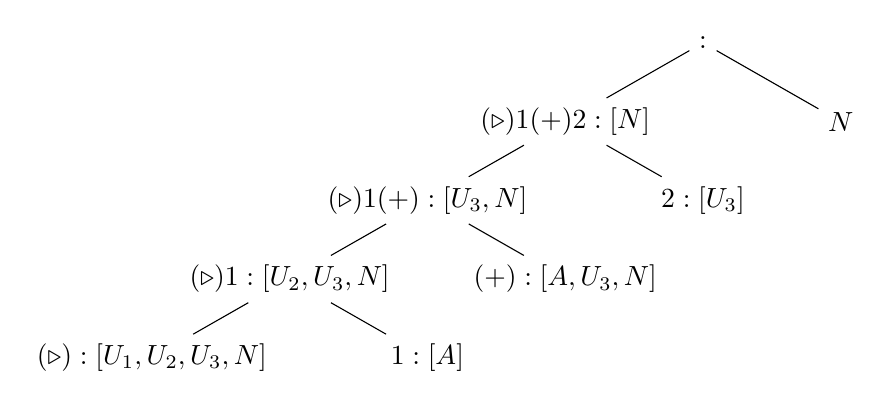
\begin{tikzpicture}
    \def\app{{\scriptsize app}}
    \def\f{{(\triangleright)}}
    \def\p{{(+)}}
    \node {:} [sibling distance = 3.5cm, level distance = 1cm]
        child {node {$\f 1 \p 2:[N]$}
            child {node {$\f 1 \p:[U_3, N]$}
                child {node {$\f 1:[U_2, U_3, N]$}
                    child {node {$\f: [U_1,U_2,U_3,N]$}}
                    child {node {$1: [A]$}}
                }
                child {node {$(+): [A,U_3,N]$}}
            }
            child {node {$2: [U_3]$}}
        }
        child {node {$N$}};
\end{tikzpicture}
}

We start with the elaboration of $(\triangleright) 1 (+) 2$ with the signature
requirement $[N]$ and the required type $N$.

\begin{itemize}
    \item The term is an application with the function term $(\triangleright) 1
        (+)$ and the argument $2$. We start the elaboration of the function term
        with the signature requirement $[U_3, N]$ and no required type.

    \item The term is again an application with the function term
        $(\triangleright) 1$ and the argument $(+)$. We start the elaboration
        of the function term with the signature requirement $[U_2, U_3, N]$ and
        no required type.

    \item The term is again an application with the function term
        $(\triangleright)$ and the argument $1$. We start the elaboration of the
        function term with the signature requirement $[U_1, U_2, U_3, N]$ and no
        required type.

    \item The term $(\triangleright)$ is a global name with the signature $[I,
        I, A, [A, P], P]$. Unification with the required signature $[U_1, U_2,
        U_3, N]$ results in
        $$
        \begin{array}{lll}
            U_1 &:=& A
            \\
            U_2 &:=& [A, U_3, N]
            \\
            P   &:=& [U_3, N]
        \end{array}
        $$
        Because of the two implicit arguments the term is elaborated as
        $(\triangleright)A P$ with the metavariables $A$ and $P$.

    \item Next the argument term $1$ has to be elaborated with the required
        signature $[A]$ and the required type $A$. This elaboration gets stuck
        on $A$, because the elaborator cannot decide the number type.

    \item Next the argument term $(+)$ is tried with the required signature $[A,
        U_3, N]$. The global name is ambiguous, but the ambiguity can be
        resolved by the result type. The signature is $[N, N, N]$. Unification
        with the required signature results in
        $$
        \begin{array}{lll}
            A &:=& N
            \\
            U_3 &:=& N
        \end{array}
        $$

    \item Now the complete term can be elaborated as
        $$
            (\triangleright) N (N \to N) \meta a (+) \meta b
        $$
        leaving the two holes $\meta a$ and $\meta b$ for the remaining
        arguments. However by unification the metavariables $\meta A$ and $\meta
        U_3$ are instantiated by $N$ and therefore the elaboration of the
        remaining arguments is unblocked and finally will succeed.
\end{itemize}
